%----------------------------------------------------------------------------------------
%	PACKAGES AND OTHER DOCUMENT CONFIGURATIONS
%----------------------------------------------------------------------------------------

\documentclass[
11pt, % The default document font size, options: 10pt, 11pt, 12pt
%oneside, % Two side (alternating margins) for binding by default, uncomment to switch to one side
francais, % ngerman for German
singlespacing, % Single line spacing, alternatives: onehalfspacing or doublespacing
%draft, % Uncomment to enable draft mode (no pictures, no links, overfull hboxes indicated)
%nolistspacing, % If the document is onehalfspacing or doublespacing, uncomment this to set spacing in lists to single
%liststotoc, % Uncomment to add the list of figures/tables/etc to the table of contents
%toctotoc, % Uncomment to add the main table of contents to the table of contents
%parskip, % Uncomment to add space between paragraphs
%nohyperref, % Uncomment to not load the hyperref package
headsepline, % Uncomment to get a line under the header
%chapterinoneline, % Uncomment to place the chapter title next to the number on one line
%consistentlayout, % Uncomment to change the layout of the declaration, abstract and acknowledgements pages to match the default layout
]{MastersDoctoralThesis} % The class file specifying the document structure

\usepackage[utf8]{inputenc} % Required for inputting international characters
\usepackage[T1]{fontenc} % Output font encoding for international characters

\usepackage{graphicx}
\graphicspath{ {./images/} }

\usepackage{mathpazo} % Use the Palatino font by default

\usepackage{amsmath}

\usepackage[backend=bibtex,style=authoryear,natbib=true]{biblatex} % Use the bibtex backend with the authoryear citation style (which resembles APA)

\addbibresource{example.bib} % The filename of the bibliography

\usepackage[autostyle=true]{csquotes} % Required to generate language-dependent quotes in the bibliography

%----------------------------------------------------------------------------------------
%	MARGIN SETTINGS
%----------------------------------------------------------------------------------------

\geometry{
	paper=a4paper, % Change to letterpaper for US letter
	inner=2.5cm, % Inner margin
	outer=3.8cm, % Outer margin
	bindingoffset=.5cm, % Binding offset
	top=1.5cm, % Top margin
	bottom=1.5cm, % Bottom margin
	%showframe, % Uncomment to show how the type block is set on the page
}

%----------------------------------------------------------------------------------------
%	INFORMATIONS
%----------------------------------------------------------------------------------------

\thesistitle{Approximation numérique d'ordre élevé de l'équation de Saint Venant} % Title
\supervisor{Thomas \textsc{Rey}} % Your supervisor's name, this is used in the title page, print it elsewhere with \supname
\examiner{} % Your examiner's name, this is not currently used anywhere in the template, print it elsewhere with \examname
\degree{} % Your degree name, this is used in the title page and abstract, print it elsewhere with \degreename
\author{Brice \textsc{Gonel} \\ Romain \textsc{Pinguet}} % Your name, this is used in the title page and abstract, print it elsewhere with \authorname
\addresses{} % Your address, this is not currently used anywhere in the template, print it elsewhere with \addressname

\subject{} % Your subject area, this is not currently used anywhere in the template, print it elsewhere with \subjectname
\keywords{} % Keywords for your thesis, this is not currently used anywhere in the template, print it elsewhere with \keywordnames
%\university{\href{https://www.univ-lille.fr}{Université de Lille}} % Your university's name and URL, this is used in the title page and abstract, print it elsewhere with \univname
%\department{\href{http://department.university.com}{Department or School Name}} % Your department's name and URL, this is used in the title page and abstract, print it elsewhere with \deptname
%\group{\href{http://researchgroup.university.com}{Research Group Name}} % Your research group's name and URL, this is used in the title page, print it elsewhere with \groupname
%\faculty{\href{http://faculty.university.com}{Faculty Name}} % Your faculty's name and URL, this is used in the title page and abstract, print it elsewhere with \facname

\AtBeginDocument{
\hypersetup{pdftitle=\ttitle} % Set the PDF's title to your title
\hypersetup{pdfauthor=\authorname} % Set the PDF's author to your name
\hypersetup{pdfkeywords=\keywordnames} % Set the PDF's keywords to your keywords
}


%----------------------------------------------------------------------------------------
%	Autres packages utiles 
%----------------------------------------------------------------------------------------

\usepackage{amsthm}
\newtheorem{prop}{Proposition}
\renewcommand{\thesection}{\arabic{section}}
\usepackage[utf8]{inputenc}
\usepackage[T1]{fontenc}


\begin{document}

\pagestyle{plain} % Default to the plain heading style until the thesis style is called for the body content

%----------------------------------------------------------------------------------------
%	TITLE PAGE
%----------------------------------------------------------------------------------------

\begin{titlepage}
\begin{center}

\vspace*{.06\textheight}

\textsc{\Large Mémoire de recherche}\\[0.5cm] % Thesis type

\HRule \\[0.4cm] % Horizontal line
{\huge \bfseries \ttitle\par}\vspace{0.4cm} % Thesis title
\HRule \\[1.5cm] % Horizontal line
 
\begin{minipage}[t]{0.4\textwidth}
\begin{flushleft} \large
\emph{Auteurs :}\\
\authorname % Author name - remove the \href bracket to remove the link
\end{flushleft}
\end{minipage}
\begin{minipage}[t]{0.4\textwidth}
\begin{flushright} \large
\emph{Professeur encadrant :} \\
\supname % Supervisor name - remove the \href bracket to remove the link  
\end{flushright}
\end{minipage}\\[3cm]
 
\end{center}
\end{titlepage}

%----------------------------------------------------------------------------------------
%	LIST OF CONTENTS/FIGURES/TABLES PAGES
%----------------------------------------------------------------------------------------

\tableofcontents % Prints the main table of contents

%----------------------------------------------------------------------------------------
%	CONTENU
%----------------------------------------------------------------------------------------

\newpage

\section{Description et dérivation des équations}

Ici, il s'agit  d'énoncer les équations, de décrire les différentes quantités en jeu ($h$, $u$, $q$ et $Z$)
et d'expliquer comment on peut arriver à ces équations.

\subsection{Description des équations}

Le système de Saint-Venant avec terme source (qui est aussi désigné par le nom \og équations d'écoulements en eau peu profonde  \fg{}) est le suivant :

$$
\left \{
\begin{array}{rcl}
\frac{\partial h}{\partial t}(t,x)&+&\frac{\partial q}{\partial x}(t,x)=0\ \\ 
\frac{\partial q}{\partial t}(t,x)&+&\frac{\partial}{\partial x}(\frac{q^{2}(t,x)}{h(t,x)}+g\frac{h^{2}(t,x)}{2})=-gh(t,x)\frac{\partial Z}{\partial x}(x) \label{deuxeq}
\end{array}
\right.
$$

\

Celui-ci permet de décrire un écoulement d'eau unidirectionnel où $h(t,x)>0$ représente la hauteur d'eau, $u(t,x)$ désigne la vitesse du fluide, $q(t,x)=h(t,x)u(t,x)$ le débit du fluide et $Z(x)$ la topographie canal ; $t\geq0$ étant le temps, $x\in\mathbb{R}$ la position spatiale dans le cours d'eau et $g$ la constante de gravitation.

\

Dans ce système, $Z$ ne dépend pas du temps $t$. On
fait ainsi l'hypothèse que le fond ne s'érode pas au cours du temps ; ce qui parait raisonnable dans de nombreuses situations (un fond rocheux sur une courte durée, par exemple).

\subsection{Dérivation des équations}

Rappelons la règle de Leibniz qui permet de calculer la dérivée par rapport à $x$ d'une fonction de la forme $\int_{a(x)}^{b(x)} f(x,t)\,~\mathrm dt$.

\begin{prop}[Règle de Leibniz]
Soit $f : \mathbb{R}^{2} \rightarrow\mathbb{R}$ telle que $f$ et ${\partial f\over\partial x}$ soient continues sur $\mathbb{R}$, et soient $a$ et $b$ deux fonctions dérivables de $\mathbb{R}$ dans $\mathbb{R}$. Alors, l'intégrale paramétrique $F$ définie sur $\mathbb{R}$ par : $F(x)=\int_{a(x)}^{b(x)}f(x,y)~\mathrm dy$ est dérivable et :
\begin{equation}
F'(x)=f(x, b(x))b'(x)-f(x,a(x))a'(x)+\int_{a(x)}^{b(x)}{\partial f\over \partial x}(x,y)~\mathrm dy.
\end{equation}
\end{prop}

Nous noterons par la suite $$\textbf{V}=\begin{bmatrix}u\\ v \\ w \end{bmatrix}$$ le vecteur dont les composantes sont les vitesses $u, v$ et $w$ dans les directions $(Ox), (Oy)$ et $(Oz)$ respectivement.

\

Nous allons maintenant dériver la deuxième équation du système. Il s'agit de l'\textbf{équation du moment}. Ecrivons la composante selon $(Ox)$ de l'équation d'Euler : 

\begin{equation}
\frac{Du}{Dt} = \frac{\partial u}{\partial t}+u\frac{\partial u}{\partial x}+v\frac{\partial u}{\partial y}+w\frac{\partial u}{\partial z}=-\frac{1}{\rho}\frac{\partial P}{\partial x}. \label{EqEulerX}
\end{equation}

On fait l'hypothèse que les quantités $h$ et $u$ sont invariantes selon l'axe $(Oy)$. Ainsi, l'étude se ramène au plan $(Oxz)$. Dans ces conditions, le terme $\frac{\partial u}{\partial y}$ est nul et on obtient :

\begin{equation}
\frac{\partial u}{\partial t}+u\frac{\partial u}{\partial x}+w\frac{\partial u}{\partial z}=-\frac{1}{\rho}\frac{\partial P}{\partial x}.
\end{equation}

La loi de conservation de la masse pour un fluide incompressible est
\begin{equation}
\text{div}(\textbf{V})=\frac{\partial u}{\partial x}+\frac{\partial v}{\partial y}+\frac{\partial w}{\partial z}=0. \label{eq:Romain}
\end{equation}

En multipliant par $u$ cette équation,
on arrive à  $u\frac{\partial u}{\partial x}+u\frac{\partial v}{\partial y}+u\frac{\partial w}{\partial z}=0$. D'où en sommant avec \eqref{EqEulerX} :

\begin{equation}
\frac{\partial u}{\partial t}+\frac{\partial}{\partial x} (u^{2})+\frac{\partial}{\partial y}(uv)+\frac{\partial }{\partial z}(uw)=-\frac{1}{\rho}\frac{\partial P}{\partial x}.
\end{equation}

De nouveau, l'hypothèse d'invariance selon $(Oy)$ permet de dire que $\frac{\partial}{\partial y}(uv)=0$ et on arrive à :
\begin{equation}
\frac{\partial u}{\partial t}+\frac{\partial}{\partial x} (u^{2})+\frac{\partial }{\partial z}(uw)=-\frac{1}{\rho}\frac{\partial P}{\partial x}.
\end{equation}

Maintenant, on intègre entre $z=Z$ et $z=Z+h$ :

\begin{equation}
\int_{Z}^{Z+h}\left[\frac{\partial u}{\partial t}+\frac{\partial }{\partial x}(u^{2})\right]~\mathrm dz+\left[uw\right]_{Z}^{Z+h}=-\frac{1}{\rho}\int_{Z}^{Z+h}\frac{\partial P}{\partial x}~\mathrm dz. \label{EqInt}
\end{equation}

Avec la règle de Leibniz, on a d'une part :

\begin{equation}
\begin{split}
& \frac{\partial}{\partial t}\int_{Z}^{Z+h}u ~\mathrm dz = \int_{Z}^{Z+h}\frac{\partial u}{\partial t} ~\mathrm dz +u\vert_{z=Z+h}\frac{\partial}{\partial t}(Z+h)-u\vert_{z=Z}\frac{\partial Z}{\partial t} \\
& = \int_{Z}^{Z+h}\frac{\partial u}{\partial t} ~\mathrm dz +u\vert_{z=Z+h}\frac{\partial h}{\partial t} \\
\end{split}
\end{equation}

la suppression du terme $\frac{\partial Z}{\partial t}$ venant du fait que la topographie est supposée constante au cours du temps.

\

Et d'autre part on a :

\begin{equation}
\frac{\partial}{\partial x}\int_{Z}^{Z+h}u^{2} ~\mathrm dz = \int_{Z}^{Z+h}\frac{\partial }{\partial x}(u^{2}) ~\mathrm dz +u^{2}\vert_{z=Z+h}\frac{\partial}{\partial x}(Z+h)-u^{2}\vert_{z=Z}\frac{\partial Z}{\partial x} 
\end{equation}

\

Donc en injectant dans \eqref{EqInt} on obtient :

\begin{equation}
\begin{split}
& \frac{\partial}{\partial t}\left[\int_{Z}^{Z+h}u ~\mathrm dz\right] -u\vert_{z=Z+h}\frac{\partial h}{\partial t} + \frac{\partial}{\partial x}\left[\int_{Z}^{Z+h} u^{2} ~\mathrm dz\right]-u^{2}\vert_{z=Z+h}\frac{\partial}{\partial x}(Z+h) \\
& +u^{2}\vert_{z=Z}\frac{\partial Z}{\partial x}+u\vert_{z=Z+h}w\vert_{z=Z+h}-u\vert_{z=Z}w\vert_{z=Z}= -\frac{1}{\rho}\int_{Z}^{Z+h}\frac{\partial P}{\partial x} ~\mathrm dz \\
\end{split}
\end{equation}


Si l'on suppose que la vitesse $u$ est constante selon l'axe $(Oz)$, on a que $\int_{Z}^{Z+h}u ~\mathrm dz = uh$ et $\int_{Z}^{Z+h}u^{2} ~\mathrm dz = u^{2}h$, et donc :

\begin{equation}
\begin{split}
& \frac{\partial}{\partial t}(uh)+ \frac{\partial}{\partial x}(u^{2}h)-u\vert_{z=Z+h}(\frac{\partial h}{\partial t}+u\vert_{z=Z+h}\frac{\partial}{\partial x}(Z+h)-w\vert_{z=Z+h}) \\
& =-\frac{1}{\rho}\int_{Z}^{Z+h}\frac{\partial u}{\partial t} ~\mathrm dz \\ \label{name}
\end{split}
\end{equation}

Or comme $\frac{\partial h}{\partial t}+u\vert_{z=Z+h}\frac{\partial}{\partial x}(Z+h)=w\vert_{z=Z+h}$, l'équation \ref{name} se réduit en

\begin{equation}
 \frac{\partial q}{\partial t}+ \frac{\partial}{\partial x}(hu^{2})=-\frac{1}{\rho}\int_{Z}^{Z+h}\frac{\partial P}{\partial x} ~\mathrm dz \label{brice2}
 \end{equation}

Encore une fois avec la règle de Leibniz 
$$\int_{Z}^{Z+h}\frac{\partial P}{\partial x} ~\mathrm dz =\frac{\partial }{\partial x}\int_{Z}^{Z+h}P ~\mathrm dz + P(Z+h)\frac{\partial}{\partial x}(Z+h)-P(Z)\frac{\partial Z}{\partial x} = \frac{\partial }{\partial x}\int_{Z}^{Z+h}P ~\mathrm dz-\rho g h\frac{\partial Z}{\partial x}.$$ 

En utilisant la formule d'équilibre hydrostatique : 
\begin{equation}
\frac{\partial}{\partial x}\int_{Z}^{Z+h}P ~\mathrm dz=\frac{\partial}{\partial x} \int_{Z}^{Z+h}\rho g(Z+h-z) ~\mathrm dz = \frac{\partial}{\partial x}(\rho g h^{2}/2) \label{brice3}
\end{equation}

Et en combinant \ref{brice2} et \ref{brice3} on arrive à la deuxième équation en rempla\c cant :

\begin{equation}
\frac{\partial q}{\partial t}+\frac{\partial}{\partial x}(\frac{q^{2}}{h}+g\frac{h^{2}}{2})=g h\frac{\partial Z}{\partial x} \label{EqSaintVenant2}
\end{equation}

%Partie Romain%

Pour obtenir la première équation, repartons de \ref{eq:Romain} et intégrons entre $z=Z$ et $z=Z+h$ :

\begin{equation}
\int_{Z}^{Z+h} (u_x + v_y) \ dz + w\vert_{z=Z+h}-w\vert_{z=Z} = 0 
\label{EqRomain1}
\end{equation}

Pour résoudre cette équation, il est nécessaire de poser ces conditions au bord :

\begin{align}
\frac{D}{Dt} (Z+h-z) = 0 \quad \text{en z = Z+h} \label{BordHaut}\\
\frac{D}{Dt} (Z-z) = 0 \quad \text{en z = Z} \label{BordBas}
\end{align}

La première condition au bord traduit l'hypothèse que la composante normale de la vitesse à la surface est nulle, autrement dit qu'il n'y a pas de flux entrant par la surface de l'eau.

\medskip

La deuxième condition au bord traduit le même phénomène mais au niveau du fond de l'eau.

\bigskip

On peut remplacer ces deux dérivées droites en temps grâce à \ref{EqEulerX} :

\begin{align}
[ \frac{\partial (Z+h)}{\partial t} + u.\frac{\partial (Z+h)}{\partial x} + v.\frac{\partial (Z+h)}{\partial y} - w ] \vert _{z=Z+h} = 0 \label{BordHautDvpt} \\
[ u.Z_x + v.Z_y + w ] \vert _{z=Z} = 0 \label{BordBasDvpt}
\end{align}

Et grâce à cette relation :

\begin{equation}
\frac{\partial}{\partial x} \int_{a(x,y)}^{b(x,y)} u \ dz = \int_{a(x,y)}^{b(x,y)} \frac{\partial u}{\partial x} \ dz + u(b(x,y)).\frac{\partial b}{\partial x} + u(a(x,y)).\frac{\partial a}{\partial x}
\end{equation}

En réinsérant \ref{BordHautDvpt} et \ref{BordBasDvpt} dans \ref{EqRomain1}, on a finalement : 

\begin{equation}
\frac{\partial (Z+h)}{\partial t} + \frac{\partial}{\partial x} \int_{Z}^{Z+h} u \ dz +  \frac{\partial}{\partial y} \int_{Z}^{Z+h} v \ dz
\end{equation}

Nous pouvons davantage simplifier cette équation en observant que u et v sont indépendants de z, ainsi que Z indépendant du temps. Cette équation devient donc :

\begin{equation}
\frac{\partial h}{\partial t} + \frac{\partial}{\partial x} (u . h ) + \frac{\partial}{\partial y} (v . h )=0 \label{EqSaintVenant1}
\end{equation}

Soit la première équation de Saint Venant.

\bigskip

Les deux équations \ref{EqSaintVenant1} et \ref{EqSaintVenant2} forment un système d'équations aux dérivées partielles d'inconnues $h$ et $q$ (ou $h$ et $u$). Etant données des conditions de bord et des conditions initiales, on doit pouvoir justifier qu'il existe une unique solution que l'on peut calculer numériquement à l'aide d'un schéma de type éléments finis.

\section{Découverte du modèle et premières propriétés qualitatives}

\begin{prop} La vitesse $u$ vérifie la loi de conservation hyperbolique scalaire suivante : 
\begin{equation}
\frac{\partial u}{\partial t}+\frac{\partial}{\partial x}(\frac{u^{2}}{2}+g(Z+h))=0 \label{cl}
\end{equation}

\end{prop}

\begin{proof}
Puisque $q=h.u$, la dérivée spatiale de $q$ s'écrit : \begin{equation}\frac{\partial q}{\partial x} = u\frac{\partial h}{\partial x}+h\frac{\partial u}{\partial x} \label{eq1}\end{equation}
et la dérivée temporelle : \begin{equation} \frac{\partial q}{\partial t} =  u\frac{\partial h}{\partial t} +  h\frac{\partial u}{\partial t} \label{eq2} \end{equation}
Alors en utilisant l'équation (mettre ici ref) du système, la dérivée temporelle donne aussi la relation \begin{equation}  \frac{\partial q}{\partial t}=-u\frac{\partial q}{\partial x}+h\frac{\partial u}{\partial t} \label{eq3}\end{equation}

\

La loi de conservation que l'on cherche à montrer est alors une réécriture de l'équation (mettre ici ref) du système. On a en effet :

$$
\frac{\partial q}{\partial t} + \frac{\partial }{\partial x}(\frac{q^{2}}{h}+g\frac{h^{2}}{2}) = -gh\frac{\partial Z}{\partial x}
$$
\

En développant la dérivée par rapport à $x$ et en utilisant \eqref{eq3} : 
$$
-u\frac{\partial q}{\partial x}+h\frac{\partial u}{\partial t}+u^{2}\frac{\partial h }{\partial x}+2hu\frac{\partial u}{\partial x} +gh\frac{\partial h}{\partial x}= -gh\frac{\partial Z}{\partial x}
$$

$$
\Leftrightarrow -u\frac{\partial q}{\partial x}+h\frac{\partial u}{\partial t}+u^{2}\frac{\partial h }{\partial x}+2hu\frac{\partial u}{\partial x} +gh\frac{\partial h}{\partial x} + gh\frac{\partial Z}{\partial x} =0
$$

$$
\Leftrightarrow u\left[-\frac{\partial q}{\partial x}+\frac{h}{u}\frac{\partial u}{\partial t}+u\frac{\partial h }{\partial x}\right]+h\left[u \frac{\partial u}{\partial x}+\frac{\partial}{\partial x}(\frac{u^{2}}{2}+g(Z+h))\right] =0
$$

$$
\Leftrightarrow u\left[-\frac{\partial q}{\partial x}+\frac{h}{u}\frac{\partial u}{\partial t}+u\frac{\partial h }{\partial x} + h\frac{\partial u }{\partial x}\right]+h\left[\frac{\partial}{\partial x}(\frac{u^{2}}{2}+g(Z+h))\right] =0
$$

\

D'après \eqref{eq1}, une simplification s'opère dans les crochets de gauche et on obtient :

$$
u\left[\frac{h}{u}\frac{\partial u}{\partial t}\right]+h\left[\frac{\partial}{\partial x}(\frac{u^{2}}{2}+g(Z+h))\right] =0
$$
\

Il suffit alors de diviser par $h>0$ pour obtenir le résultat \eqref{cl}.

\end{proof}

\section{Implémentation du schéma de Rusanov}

\subsection{Présentation du schéma et résultats de convergence}

Dans cette partie, il s'agit de résoudre numériquement le système de Saint-Venant. 
Posons

\begin{center}

$\textbf{U}=\begin{pmatrix}
   h \\
    q \\
\end{pmatrix}\in\mathbb{R}^{2},  \phantom{..} \textbf{F} (\textbf{U}) =\begin{pmatrix}
   q \\
   \frac{q^{2}}{h}+g\frac{h^{2}}{2} \\
\end{pmatrix}\in\mathbb{R}^{2} \phantom{..} \text{et} \phantom{...} \textbf{B} (\textbf{U}) =\begin{pmatrix}
   0 \\
   -gh \frac{\partial Z}{\partial x}\\
\end{pmatrix}\in\mathbb{R}^{2}.
$
\end{center}

$\textbf{U}$ désigne le vecteur inconnu, $\textbf{F} (\textbf{U})$ la fonction flux et $\textbf{B} (\textbf{U})$ le terme source. Avec ces notations,
le système de départ se réécrit $$\frac{\partial\textbf{U}}{\partial t}+\frac{\partial}{\partial x}(\textbf{F} (\textbf{U})) = \textbf{B} (\textbf{U})$$

\begin{prop}
Posons le vecteur $\textbf{W}= (h, u)^{T}$ (variable dite non conservative). $\textbf{W}$ vérifie le système quasi-linéaire suivant :
$$ \frac{\partial \textbf{W}}{\partial t} +\mathbb{A}(\textbf{W}) \frac{\textbf{W}}{\partial x} = 0 \label{ql} $$
avec $\mathbb{A}(\textbf{W})$ définie par :

$$\mathbb{A}(\textbf{W}) =\begin{pmatrix}
   u & h  \\
   g & u  \\
\end{pmatrix}$$

\end{prop}

\begin{proof}

\end{proof}

\begin{prop}
La matrice $\mathbb{A}(\textbf{W})$ est diagonalisable et on a :
$$
\mathbb{P}(\textbf{W})^{-1}\mathbb{A}(\textbf{W})\mathbb{P}(\textbf{W})=\mathbb{D}(\textbf{W})
$$
où 

\begin{center}

$\mathbb{D}(\textbf{W}) =\begin{pmatrix}
   u+\sqrt{gh} & 0  \\
   0 & u-\sqrt{gh}  \\
\end{pmatrix} \phantom{..} \text{et}\phantom{...} \mathbb{P}(\textbf{W}) =\begin{pmatrix}
   \frac{\sqrt{h}}{\sqrt{g}} & -\frac{\sqrt{h}}{\sqrt{g}} \\
   1 & 1  \\
\end{pmatrix}.
$
\end{center}

\end{prop}

\begin{proof} Le résultat est direct en faisant le produit matriciel si on connait les expressions de $\mathbb{D}(\textbf{W})$ et $\mathbb{P}(\textbf{W})$. Dans le cas contraire, on procède comme suit :

\

On détermine les valeurs propres de la matrice $\mathbb{A}(\textbf{W})$, ce qui conduit à chercher les racines du polynôme (d'indéterminée $\lambda$) suivant :

$$\det(\mathbb{A}(\textbf{W})-\lambda I) =\begin{vmatrix}
   u-\lambda & h  \\
   g & u-\lambda  \\
\end{vmatrix} = (u-\lambda)^{2}-gh.$$

Or puisque $g$ et $h$ sont $>0$,

$$(u-\lambda)^{2}-gh=0 \Leftrightarrow \lambda u +\sqrt{gh} \phantom{...}\text{ou}\phantom{...} \lambda u -\sqrt{gh}$$

et comme la matrice admet deux valeurs propres distinctes, elle est diagonalisable. La matrice diagonale est alors

$$\mathbb{D}(\textbf{W}) =\begin{pmatrix}
   u+\sqrt{gh} & 0  \\
   0 & u-\sqrt{gh}  \\
\end{pmatrix}.
$$

\

Il reste à déterminer la matrice de passage $\mathbb{P}(\textbf{W})$. Il s'agit de trouver 
$\begin{pmatrix}
   a\\
   b\\
\end{pmatrix}
$ un vecteur propre associé à $u +\sqrt{gh}$ et
$\begin{pmatrix}
   c\\
   d\\
\end{pmatrix}
$ un vecteur propre associé à $u -\sqrt{gh}$.

\

\underline{Pour le vecteur propre associé à $u +\sqrt{gh}$ :}

\

$$\mathbb{A}(\textbf{W}) \begin{pmatrix}
   a\\
   b\\
\end{pmatrix}=\begin{pmatrix}
   u & h  \\
   g & u  \\
\end{pmatrix} \begin{pmatrix}
   a\\
   b\\
\end{pmatrix}=(u+\sqrt{gh})\begin{pmatrix}
   a\\
   b\\
\end{pmatrix}$$

\

Il s'agit d'un système lié donc il est équivalent de raisonner sur la première équation :

$$au+bh = au+ a\sqrt{gh}$$

$$\Leftrightarrow bh = a\sqrt{gh}$$

\

et on voit que $\begin{pmatrix}
   a\\
   b\\
\end{pmatrix} = \begin{pmatrix}
   \sqrt{h}/\sqrt{g}\\
   1\\
\end{pmatrix}$ convient.

\

De même, \underline{pour le vecteur propre associé à $u -\sqrt{gh}$ :}

\

Cette fois on arrive à $$cu+dh = cu- c\sqrt{gh}$$

$$\Leftrightarrow dh = -c\sqrt{gh}$$

\

et on voit que $\begin{pmatrix}
   c\\
   d\\
\end{pmatrix} = \begin{pmatrix}
   -\sqrt{h}/\sqrt{g}\\
   1\\
\end{pmatrix}$ convient.

\

D'où finalement : $$\mathbb{P}(\textbf{W}) =\begin{pmatrix}
   \frac{\sqrt{h}}{\sqrt{g}} & -\frac{\sqrt{h}}{\sqrt{g}} \\
   1 & 1  \\
\end{pmatrix}.$$

\end{proof}


\begin{prop}

La matrice jacobienne de $\textbf{F}$ admet deux valeurs propres distinctes $\lambda_{1}(\textbf{U})$ et $\lambda_{2}(\textbf{U})$  qui sont égales aux valeurs 
propres de $\mathbb{A}(\textbf{W}).$

\end{prop}

\begin{proof}

La matrice jacobienne de \textbf{F} est la suivante :

$$J_{\textbf{F}}(h, q) =\begin{pmatrix}
   0 & 1  \\
   -\frac{q^{2}}{h^{2}}+gh & \frac{2q}{h}  \\
\end{pmatrix}$$

\

Pour déterminer les valeurs propres de cette matrice, il faut calculer les racines du polynôme donné par

$$\det (J_{\textbf{F}}(h, q)) =\begin{vmatrix}
   0-\lambda & 1  \\
   -\frac{q^{2}}{h^{2}}+gh & \frac{2q}{h}-\lambda  \\
\end{vmatrix}$$

et $$-\lambda(\frac{2q}{h}-\lambda)+\frac{q^{2}}{h^{2}}-gh=0$$
$$\Leftrightarrow \lambda^{2}-2u\lambda+u^{2}-gh=0.$$

\

Puisque $\Delta=4u^{2}-4(u^{2}-gh)=4gh>0\phantom{.}$, il y a deux racines distinctes 
$$\lambda_{1}(\textbf{U})=\frac{2u+2\sqrt{gh}}{2} \phantom{..}\text{et}\phantom{..} \lambda_{2}(\textbf{U})=\frac{2u-2\sqrt{gh}}{2}.$$
En simplifiant par 2 au numérateur et dénominateur, on voit qu'il s'agit des valeurs propres de  $\mathbb{A}(\textbf{W}).$

\end{proof}

Dans la mesure ou la matrice jacobienne du flux a deux valeurs propres différentes, on peut appliquer le schéma de Rusanov.
Cf l'énoncé du TP. Mais il faudrait pouvoir expliquer pourquoi.

\subsection{Validation de l'implémentation avec des tests}

Dans cette partie, nous allons effectuer des tests sur notre implémentation.

\

D’abord nous allons observer numériquement la convergence de la solution numérique. Nous allons voir que lorsque le nombre $N$ grandit, 
les courbes de $h$ et $q$ on tendance à se rapprocher d’une courbe limite. Au passage, on pourra observer ce qui semble être un effet régularisant de l'équation : même lorsque l'on prend un profil initial non dérivable pour la hauteur d'eau $h$, la solution se lisse (immédiatement ?). Cette propriété devra être vérifiée. On pourra essayer de la justifier si elle est vraie...

\

Puis nous regarderons l’influence du pas spatial. En particulier, nous verrons ce qu'il se passe lorsque la condition CFL n'est pas vérifiée.

\

Enfin, nous allons confronter nos résultats à des tests que l’on retrouve fréquemment dans la littérature (rupture de barrage, bosse d’eau, etc).

\newpage

\subsubsection{Influence du pas spatial et convergence de la solution}


\begin{figure}[h]
\begin{center}$
\begin{array}{ccc}
\includegraphics[scale = .15]{"deltaT=.5 tau t=0 N=16.png"} &
\includegraphics[scale = .15]{"deltaT=.5 tau t=0 N=64.png"} &
\includegraphics[scale = .15]{"deltaT=.5 tau t=0 N=256.png"}
\\
\includegraphics[scale = .15]{"deltaT=.5 tau t=10 N=16.png"} &
\includegraphics[scale = .15]{"deltaT=.5 tau t=10 N=64.png"} &
\includegraphics[scale = .15]{"deltaT=.5 tau t=10 N=256.png"}
\\
\includegraphics[scale = .15]{"deltaT=.5 tau t=20 N=16.png"} &
\includegraphics[scale = .15]{"deltaT=.5 tau t=20 N=64.png"} &
\includegraphics[scale = .15]{"deltaT=.5 tau t=20 N=256.png"}
\\
\includegraphics[scale = .15]{"deltaT=.5 tau t=30 N=16.png"} &
\includegraphics[scale = .15]{"deltaT=.5 tau t=30 N=64.png"} &
\includegraphics[scale = .15]{"deltaT=.5 tau t=30 N=256.png"}
\end{array}$
\end{center}
\caption{Simulations pour $N$ $=$ $16,$ $64$ et $256$}
\end{figure}





\subsubsection{Influence du pas temporel}

Voici des représentations de la solution à différents instants (approximativement $t=0, 5, 10, 15$ et $20$ secondes) avec pas de temps égal $0.5\tau, \tau$ et $2\tau$ ; $\tau$ étant défini par ...

\begin{center}
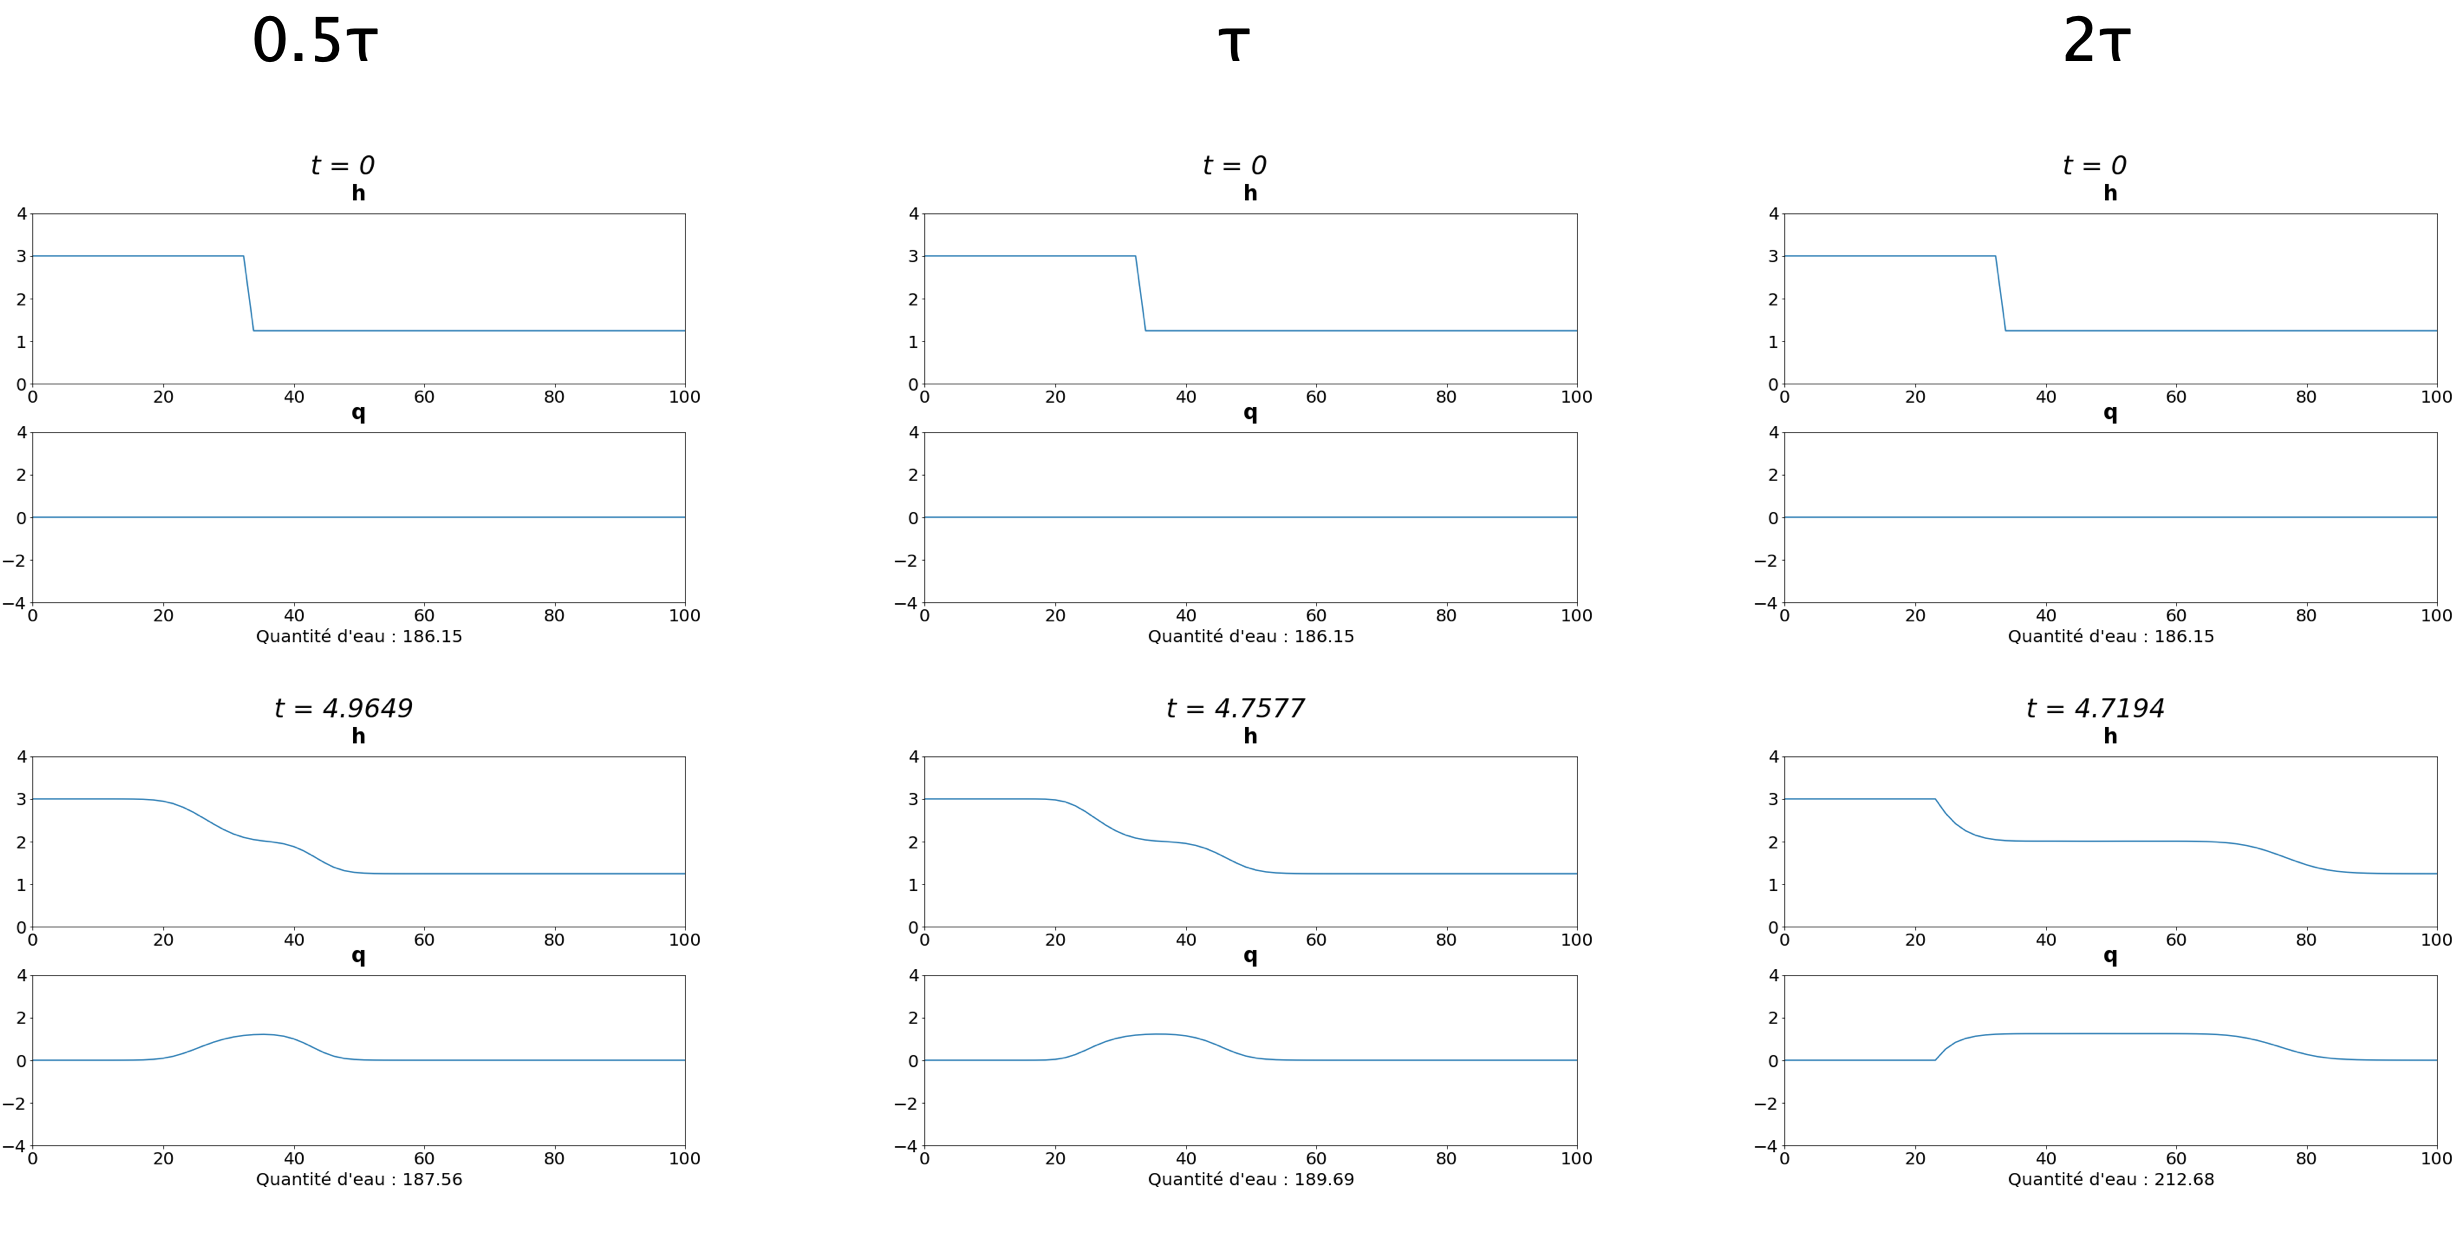
\includegraphics[scale=0.35]{part1.png} 

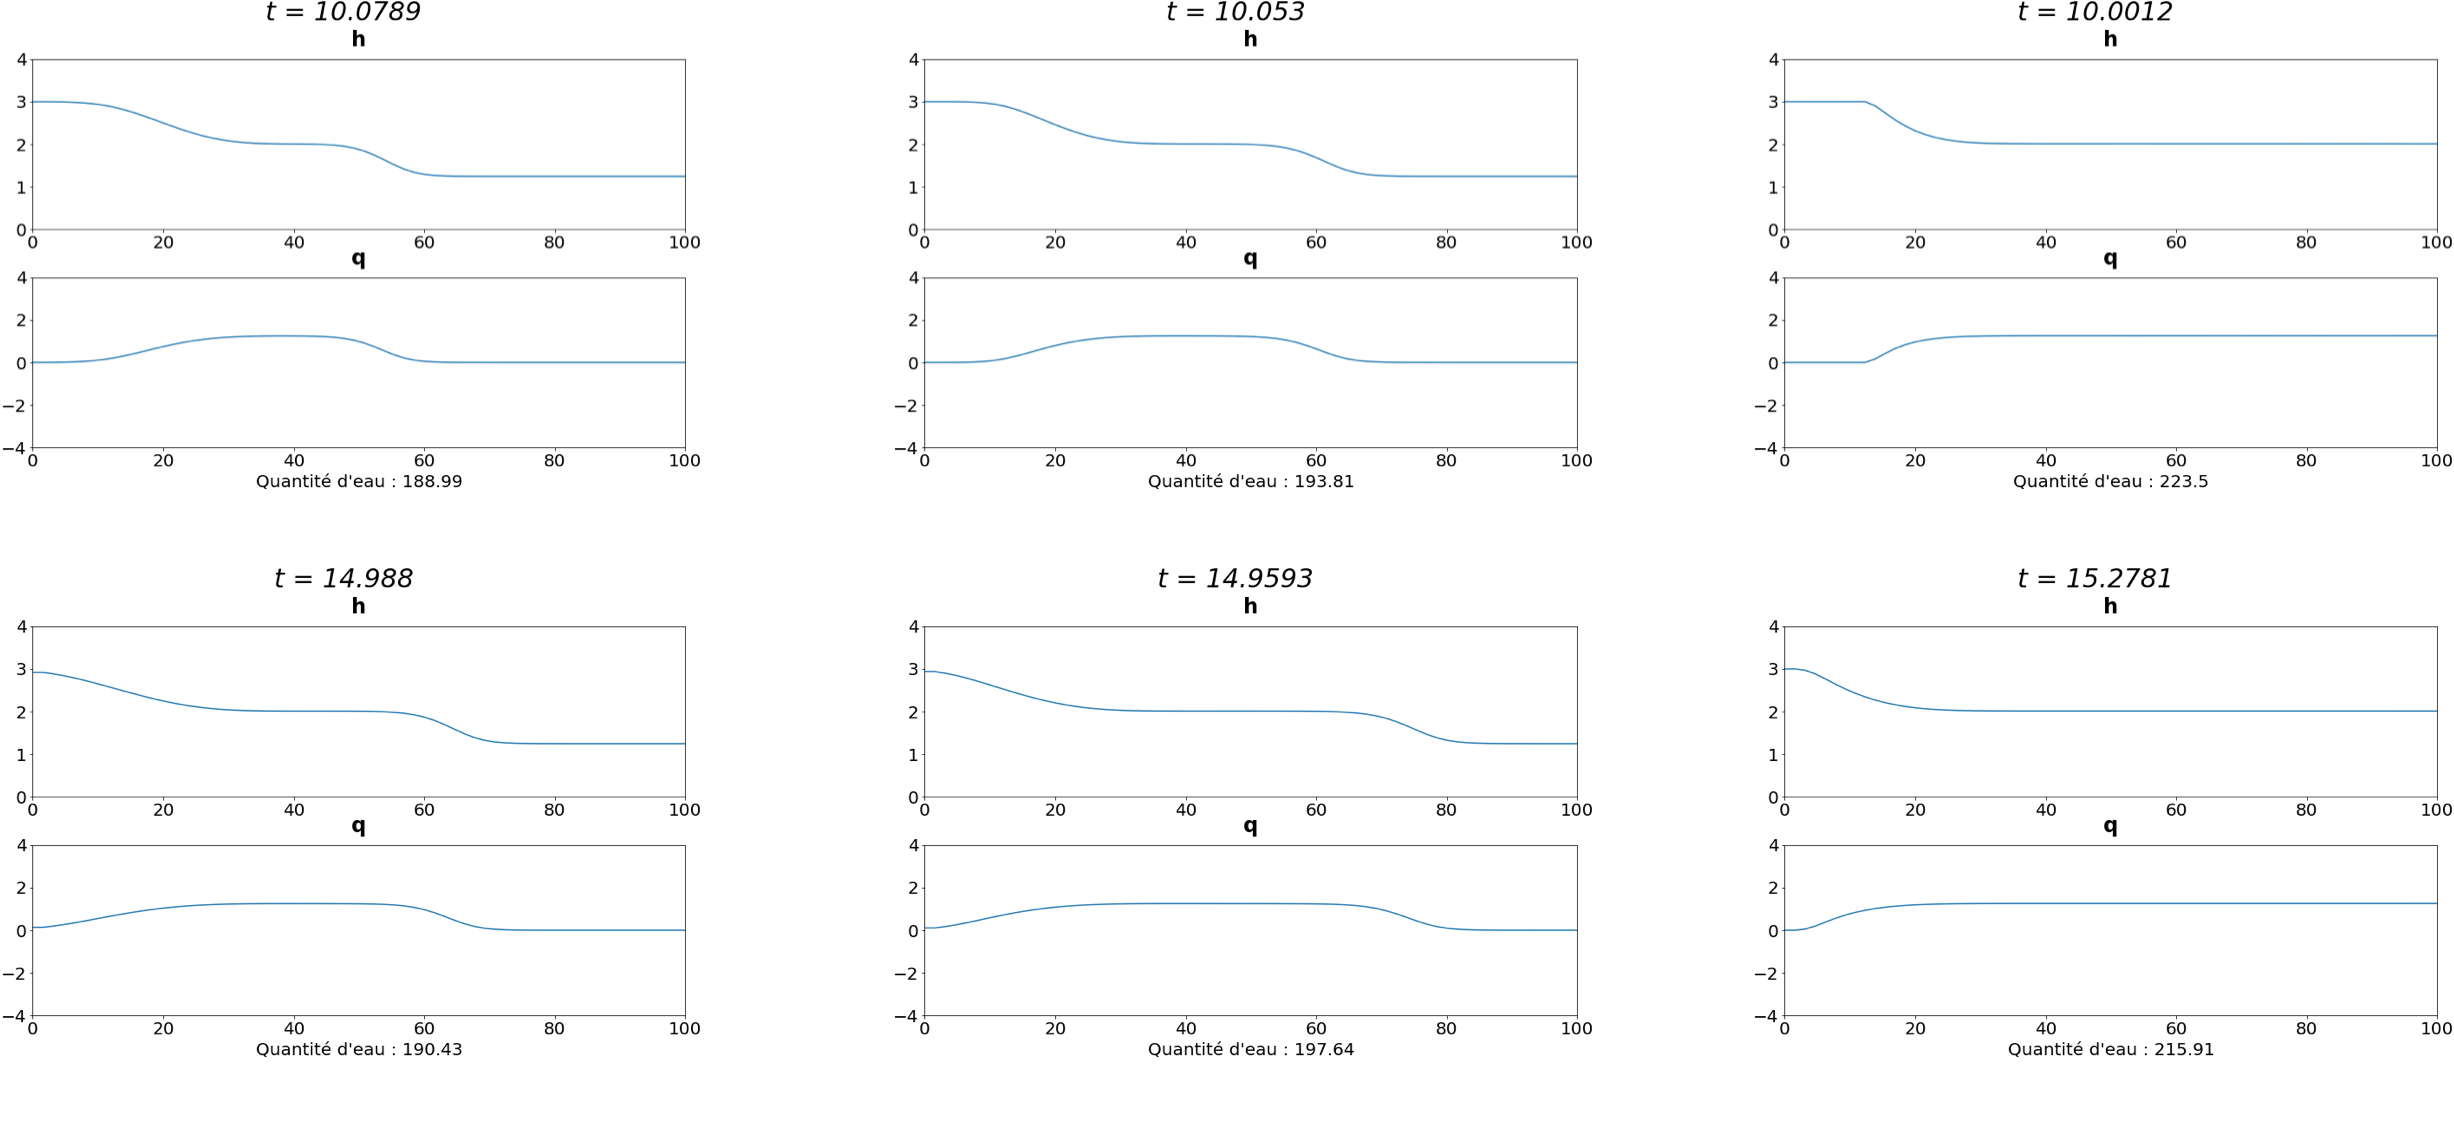
\includegraphics[scale=0.35]{part2.png} 

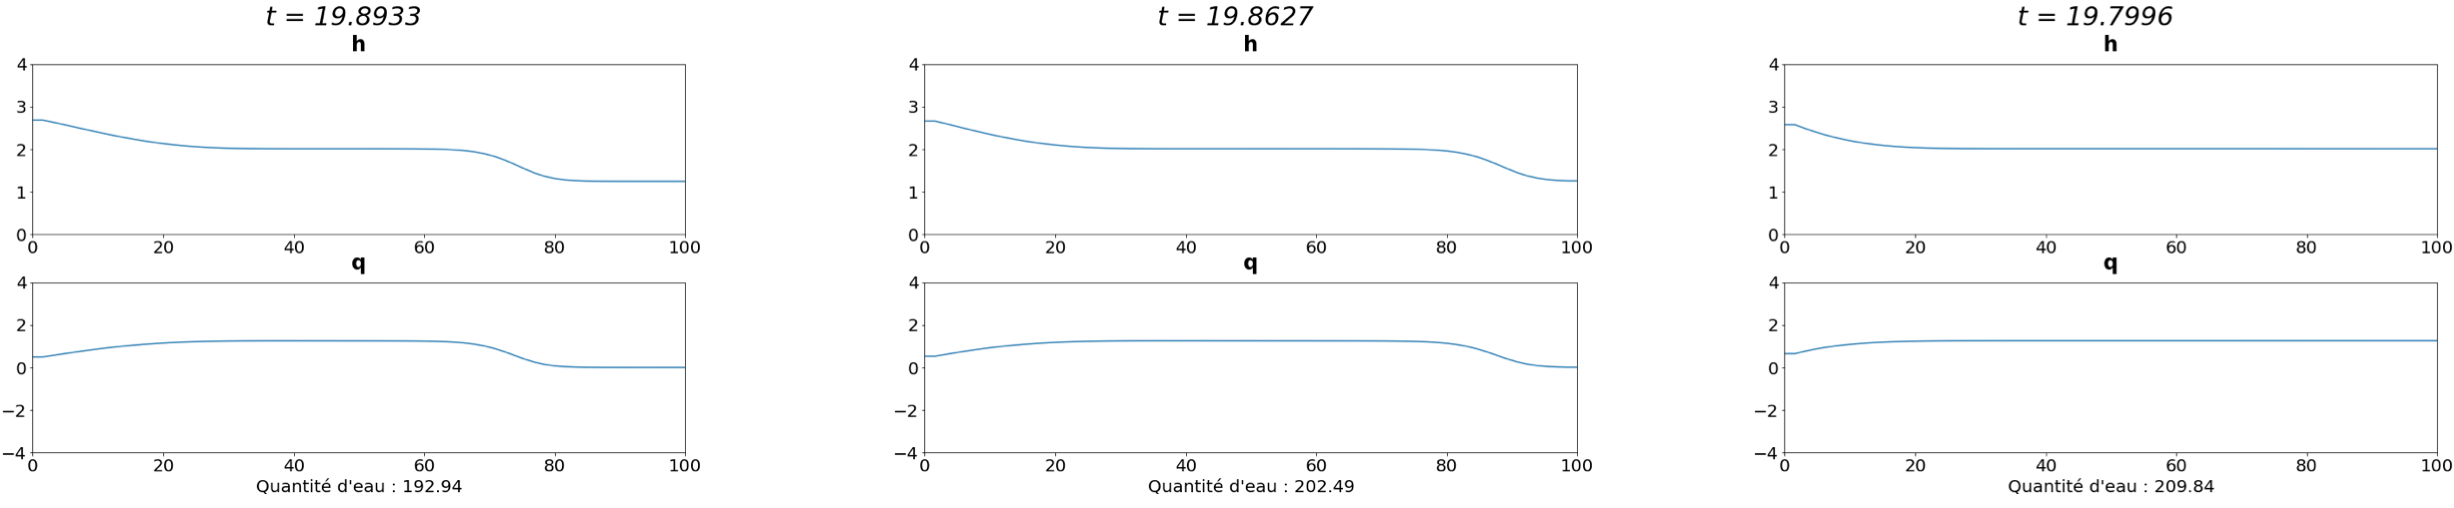
\includegraphics[scale=0.35]{part3.png} 
\end{center}

\

On remarque immédiatement l'influence du pas temporel sur la conservation de la quantité d'eau. Plus le pas est choisi petit et meilleure est la conservation. On observe une dynamique similaire pour les deux cas qui respectent la condition CFL ($\tau$ et $0.5\tau$). Néanmoins, les évolutions sont trop différentes (la vague issue de la rupture de barrage se déplace plus lentement lorsque le pas de temps est $0.5\tau$ ; cette différence vient peut être du fait que la condition doit être respectée strictement... à éclaircir). Lorsque la condition CFL n'est pas vérifiée, l'évolution est très différente.

\

On retrouve le même phénomène dans le cas de la goutte d'eau qui tombe au centre du repère : voici les mêmes représentations pour $t=0, 10, 20, 30$ secondes, avec un pas de temps égal à $0.5\tau, \tau$ et $2\tau$.

\begin{figure}[h]
\begin{center}$
\begin{array}{ccc}
\includegraphics[scale = .15]{"deltaT=.5 tau t=0 N=64.png"} &
\includegraphics[scale = .15]{"deltaT=.5 tau t=0 N=64.png"} &
\includegraphics[scale = .15]{"deltaT=.5 tau t=0 N=64.png"}
\\
\includegraphics[scale = .15]{"deltaT=.5 tau t=10 N=64.png"} &
\includegraphics[scale = .15]{"deltaT=tau t=10 N=64.png"} &
\includegraphics[scale = .15]{"deltaT=2tau t=10 N=64.png"}
\\
\includegraphics[scale = .15]{"deltaT=.5 tau t=20 N=64.png"} &
\includegraphics[scale = .15]{"deltaT=tau t=20 N=64.png"} &
\includegraphics[scale = .15]{"deltaT=2tau t=20 N=64.png"}
\\
\includegraphics[scale = .15]{"deltaT=.5 tau t=30 N=64.png"} &
\includegraphics[scale = .15]{"deltaT=tau t=30 N=64.png"} &
\includegraphics[scale = .15]{"deltaT=2tau t=30 N=64.png"}
\end{array}$
\end{center}
\caption{Simulations pour différentes valeurs de $\tau$}
\end{figure}

\

De même, plus le pas temporel est faible, plus la quantité d'eau est conservée au cours du temps. On remarque aussi que la quantité d'eau est bien conservée quand la vague est au centre du repère. Cependant, quand elle atteint le bord et disparait aux limites, la quantité d'eau baisse brutalement ( il suffit de comparer la quantité entre $t=0\ s$ et $t=20\ s$ puis la quantité entre $t=20\ s$ et $t=30\ s$ ). 

\

\subsubsection{Confrontation de l'implémentation à des références}





\section{Utilisation des limiteurs de pente pour une montée en ordre}

\section{Passage au cas 2D}

\newpage
\renewcommand{\thesection}{\Alph{section}}
\appendix
\section{Annexes}
\subsection{Le code}


%----------------------------------------------------------------------------------------
%	BIBLIOGRAPHY
%----------------------------------------------------------------------------------------

\begin{thebibliography}{9}

\bibitem{RL} R. \textsc{Leveque},
\textit{Finite Volume Methods for Hyperbolic Problems}, Cambridge University Press, 2004

\bibitem{ET} E. \textsc{Toro},
\textit{Riemann Solvers and Numerical Methods for Fluid Dynamic}, Springer, 2009

\bibitem{W} \textsc{Wikipedia},
\href{https://fr.wikipedia.org/wiki/Intégrale_paramétrique#Dérivabilité}{ \textit{Intégrale paramétrique}}

\end{thebibliography}

%----------------------------------------------------------------------------------------

\end{document}  

